%package list
\documentclass{article}
\usepackage[top=3cm, bottom=3cm, outer=3cm, inner=3cm]{geometry}
\usepackage{graphicx}
\usepackage{url}
%\usepackage{cite}
\usepackage{hyperref}
\usepackage{array}
\usepackage{multicol}
\newcolumntype{x}[1]{>{\centering\arraybackslash\hspace{0pt}}p{#1}}
\usepackage{natbib}
\usepackage{pdfpages}
\usepackage{multirow}
\usepackage{float}
\usepackage[normalem]{ulem}
\useunder{\uline}{\ul}{}
\usepackage{svg}
\usepackage{amsmath}
\usepackage{hyperref}

%%%%%%%%%%%%%%%%%%%%%%%%%%%%%%%%%%%%%%%%%%%%%%%%%%%%%%%%%%%%%%%%%%%%%%%%%%%%
%%%%%%%%%%%%%%%%%%%%%%%%%%%%%%%%%%%%%%%%%%%%%%%%%%%%%%%%%%%%%%%%%%%%%%%%%%%%
\newcommand{\csemail}{vmachacaa@unsa.edu.pe}
\newcommand{\csdocente}{Vicente Machaca Arceda}
\newcommand{\cscurso}{Algoritmos y Estructura de Datos}
\newcommand{\csuniversidad}{Universidad Nacional de San Agustín}
\newcommand{\csescuela}{Maestría en Ciencias de la Computación}
\newcommand{\cspracnr}{02}
\newcommand{\cstema}{Estructura de datos}
%%%%%%%%%%%%%%%%%%%%%%%%%%%%%%%%%%%%%%%%%%%%%%%%%%%%%%%%%%%%%%%%%%%%%%%%%%%%
%%%%%%%%%%%%%%%%%%%%%%%%%%%%%%%%%%%%%%%%%%%%%%%%%%%%%%%%%%%%%%%%%%%%%%%%%%%%


\usepackage[english,spanish]{babel}
\usepackage[utf8]{inputenc}
\AtBeginDocument{\selectlanguage{spanish}}
\renewcommand{\figurename}{Figura}
\renewcommand{\refname}{Referencias}
\renewcommand{\tablename}{Tabla} %esto no funciona cuando se usa babel
\AtBeginDocument{%
	\renewcommand\tablename{Tabla}
}

\usepackage{fancyhdr}
\pagestyle{fancy}
\fancyhf{}
\setlength{\headheight}{30pt}
\renewcommand{\headrulewidth}{1pt}
\renewcommand{\footrulewidth}{1pt}
\fancyhead[L]{\raisebox{-0.2\height}{
\includegraphics[width=3cm]{img/logo_unsa}}}
\fancyhead[C]{}
\fancyhead[R]{\fontsize{7}{7}\selectfont	\csuniversidad \\ \csescuela \\ \textbf{\cscurso} }
\fancyfoot[L]{Grupo N 02}
\fancyfoot[C]{\cscurso}
\fancyfoot[R]{Página \thepage}


\begin{document}
	
	\vspace*{10px}
	
	\begin{center}	
		\fontsize{17}{17} \textbf{ Práctica \cspracnr}
	\end{center}
	%\centerline{\textbf{\underline{\Large Título: Informe de revisión del estado del arte}}}
	%\vspace*{0.5cm}
	

	\begin{table}[h]
		\begin{tabular}{|x{4.7cm}|x{4.8cm}|x{4.8cm}|}
			\hline
			\textbf{DOCENTE} & \textbf{CARRERA}  & \textbf{CURSO}   \\
			\hline
			\csdocente & \csescuela & \cscurso    \\
			\hline
		\end{tabular}
	\end{table}	
	
	
	\begin{table}[h]
		\begin{tabular}{|x{4.7cm}|x{4.8cm}|x{4.8cm}|}
			\hline
			\textbf{PRÁCTICA} & \textbf{TEMA}  & \textbf{DURACIÓN}   \\
			\hline
			\cspracnr & \cstema & --   \\
			\hline
		\end{tabular}
	\end{table}
	
	\section{Integrantes}
        	\begin{itemize}
        		\item Grupo N 2
        		\item Integrantes:
        		\begin{itemize}
        			\item EDER ALONSO, AMPUERO ATAMARI
        			\item HOWARD FERNANDO, ARANZAMENDI MORALES
        			\item JOSE EDISON, PEREZ MAMANI
        			\item HENRRY IVAN, ARIAS MAMANI
        		\end{itemize}		
        	\end{itemize}
    \section{Repositorio GitHub}
           URL Github: \href{https://github.com/hAriasm/Practica2_ayed}{Repositorio Práctica 2 AyED}
	\section{Estructuras de Datos}
   \subsection{AVL}
        \paragraph{}
        El árbol AVL recibe su nombre de las iniciales  de sus inventores, Georgii Adelson-Velskii y Yevgeniy Landis. Dieron a conocer esto mediante la publicación de un artículo en 1962, " Un algoritmo para organizar la información" (" Un algoritmo para organizar la información").

        Un árbol AVL es un árbol de búsqueda binaria que tiene una altura equilibrada: para cada nodo x, las alturas de los subárboles izquierdo y derecho de x difieren en 1 como máximo. Para implementar un árbol AVL, mantenemos un atributo adicional en cada nodo: x.h es la altura del nodo x. Como para cualquier otro árbol binario de búsqueda T, asumimos que T.root apunta al nodo raíz.

        El árbol AVL siempre está equilibrado de  modo que para todos los nodos, la altura de la rama izquierda no difiera en más de una unidad de la altura de la rama derecha o viceversa. Gracias a esta forma de equilibrio, la complejidad de una búsqueda en uno de estos árboles se mantiene siempre en el orden de complejidad O(log n). El factor de equilibrio puede almacenarse directamente en cada nodo o calcularse a partir de la altura de los subárboles.

        Para lograr este equilibrio, la inserción y eliminación de  nodos debe realizarse de manera especial. Si la condición de equilibrio se rompe al realizar una operación de inserción o eliminación, se debe realizar una serie de rotaciones de  nodos.


         \subsubsection{Resultados del experimento}
         \begin{itemize}
            \item En la figura \ref{fig:avlBusqueda} mostramos la búsqueda del nodo 22 con resultado de no encontrado
           \item En la figura \ref{fig:avlBusqueda} mostramos la búsqueda del nodo 21 con resultado de "Se encontró el nodo".
           \item En la figura \ref{fig:avlBusqueda} mostramos el máximo y  mínimo valor .
           \item En la figura \ref{fig:avlInicial} mostramos nuestro árbol inicial con 11 nodos.
           \item En la figura \ref{fig:avlIsertion} mostramos el árbol luego de insertar un nodo nuevo.
           \item En la figura \ref{fig:avldelete} mostramos luego de eliminar un nodo.
           \item En la figura \ref{fig:avldelete2} mostramos luego de eliminar el nodo raíz.
         \end{itemize}

         \begin{figure}[htbp]
              \centering
              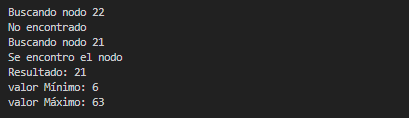
\includegraphics[width=\textwidth]{img/busquedaAVL.png}
              \caption{Árbol AVL búsqueda variada}
              \label{fig:avlBusqueda}
            \end{figure}
            \begin{figure}[htbp]
              \centering
              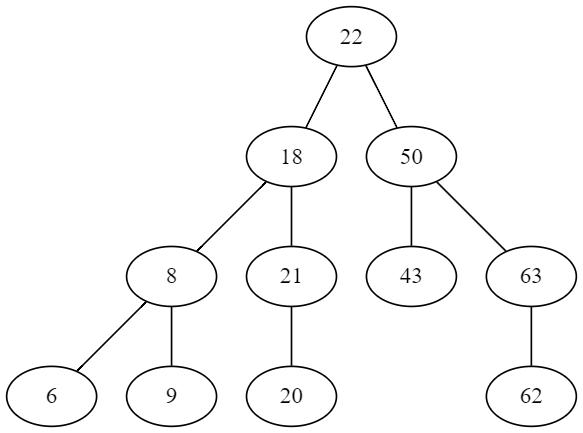
\includegraphics[width=0.5\textwidth]{img/avltree.png}
              \caption{Árbol AVL inicial}
              \label{fig:avlInicial}
            \end{figure}
            \begin{figure}[htbp]
              \centering
              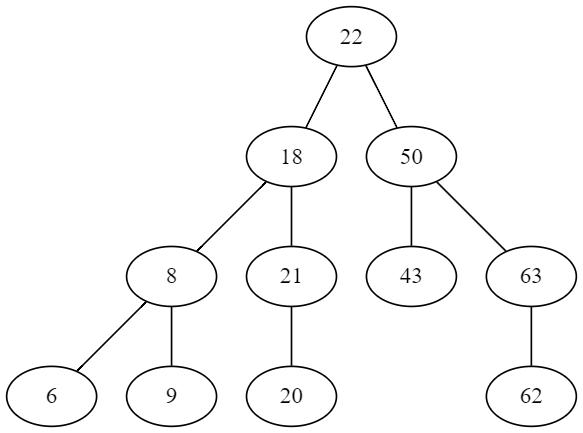
\includegraphics[width=0.5\textwidth]{img/avltree.png}
              \caption{Árbol AVL inicial}
              \label{fig:avlInicial}
            \end{figure}
            \begin{figure}[htbp]
              \centering
              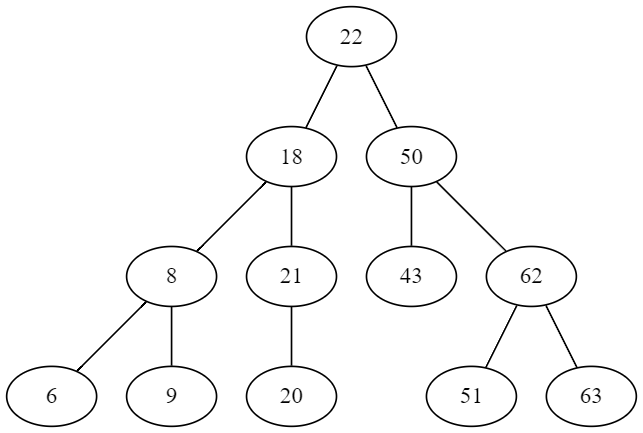
\includegraphics[width=0.5\textwidth]{img/avltree-insertion.png}
              \caption{Árbol AVL con inserción }
                \label{fig:avlIsertion}
            \end{figure}
            \begin{figure}[htbp]
              \centering
              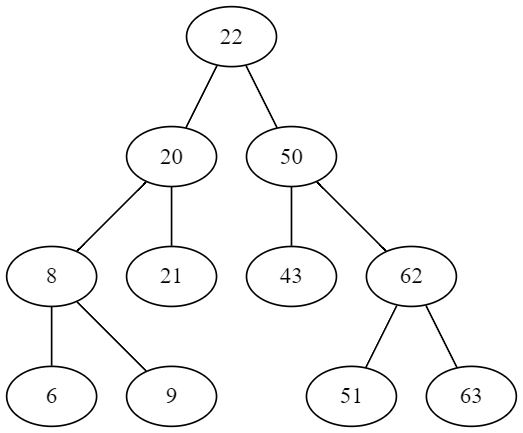
\includegraphics[width=0.5\textwidth]{img/avltree-deletion.png}
              \caption{Árbol AVL con eliminación nodo}
            \label{fig:avldelete}
            \end{figure}
             \begin{figure}[htbp]
              \centering
              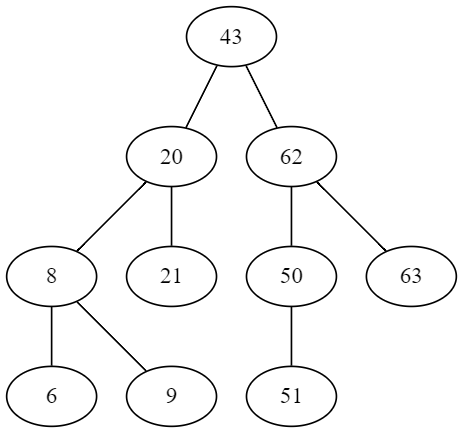
\includegraphics[width=0.5\textwidth]{img/avltree-deletion-2.png}
              \caption{Árbol AVL con eliminación de la raíz}
              \label{fig:avldelete2}
            \end{figure}
        \subsection{B-Tree}
            \paragraph{}
            La idea tras los árboles-B es que los nodos internos deben tener un número variable de nodos hijo dentro de un rango predefinido. Cuando se inserta o se elimina un dato de la estructura, la cantidad de nodos hijo varía dentro de un nodo. Para que siga manteniéndose el número de nodos dentro del rango predefinido, los nodos internos se juntan o se parten. Dado que se permite un rango variable de nodos hijo, los árboles-B no necesitan rebalancearse tan frecuentemente como los árboles binarios de búsqueda auto-balanceables. Pero, por otro lado, pueden desperdiciar memoria, porque los nodos no permanecen totalmente ocupados. Los límites (uno superior y otro inferior) en el número de nodos hijo son definidos para cada implementación en particular
            Un árbol-B se mantiene balanceado porque requiere que todos los nodos hoja se encuentren a la misma altura.
            Operaciones Básicas
                   \begin{figure}[htbp]
              \centering
              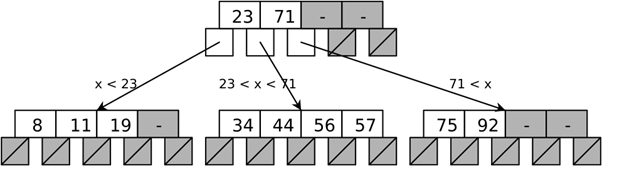
\includegraphics[width=\textwidth]{img/btree22.png}
              \caption{Gráfica B-tree}
              \label{fig:avlBusqueda}
            \end{figure}
            \textbf{Buscar:}
            La búsqueda es similar a la de los árboles binarios. Básicamente, empieza comprobando el nodo raíz, y si este es el que se busca, termina la operación. Si no lo es, mueve el puntero a su hijo izquierdo o al derecho, dependiendo de si el dato que se busca es menor o mayor del que contiene el nodo padre. De esta forma continua hasta encontrar el dato o terminar de recorrer el árbol sin encontrarlo. Este proceso es recursivo, puesto que el puntero se mueve hasta un nodo hijo, y podemos considerar a este como el nodo raíz de un nuevo árbol. El costo computacional es O($Log_2n$))
            \textbf{Insertar:}
            Las inserciones se hacen en los nodos hoja.
            \begin{itemize}
              \item  	Realizando una búsqueda en el árbol, se halla el nodo hoja en el cual debería ubicarse el nuevo elemento.
              \item Si el nodo hoja tiene menos elementos que el máximo número de elementos legales, entonces hay lugar para uno más. Inserte el nuevo elemento en el nodo, respetando el orden de los elementos.
              \item De otra forma, el nodo debe ser dividido en dos nodos.
            \end{itemize}

                \textbf{Eliminar:}
                La eliminación de un elemento es directa si no se requiere corrección para garantizar sus propiedades. Hay dos estrategias populares para eliminar un nodo de un árbol B.
                \begin{itemize}
                  \item localizar y eliminar el elemento, y luego corregir, o
                  \item hacer una única pasada de arriba abajo por el árbol, pero cada vez que se visita un nodo, reestructurar el árbol para que cuando se encuentre el elemento a ser borrado, pueda eliminarse sin necesidad de continuar reestructurando
                \end{itemize}
                Se pueden dar dos problemas al eliminar elementos. Primero, el elemento puede ser un separador de un nodo interno. Segundo, puede suceder que al borrar el elemento número de elementos del nodo quede debajo de la cota mínima

            \subsubsection{Resultados del experimento}

        \begin{itemize}
            \item   Árbol Principal
            \item   Insertar dos nodos
            \item   Borrar un nodo con dos hijos
            \item   Borrar nodo raíz
            \item   Búsqueda de un nodo
            \item	Búsqueda del mínimo
            \item	Búsqueda del máximo
        \end{itemize}
    \section{Conclusiones}
        \begin{itemize}
                 \item Un árbol AVL se mantiene ordenado, pero hay mas rotaciones en las inserciones que en las eliminaciones, su costo para buscar, eliminar, insertar  es de O(Log n).
                 \item Funciona de manera casi instantánea incluso con grandes volúmenes de datos. Ello se debe principalmente a la característica equilibrada del árbol, lo que permite tener acceso a todos los elementos con el mismo número de etapas, y en segundo lugar, al crecimiento logarítmico de la profundidad del árbol. Eso significa que la profundidad del árbol crece lentamente en comparación al número de hojas. Hay índices reales con millones de registros que tienen una profundidad de cuatro o cinco. Es poco común encontrar una profundidad de seis
        \end{itemize}

    \section{Referencias}
  \begin{enumerate}
    \item González, A. H. (2013). Operaciones sobre árboles.
    \item	Weiss, M. A., Jorge tr Lozano Moreno, Andoni colab. téc Eguíluz,   Inés colab. téc Jacob. (1995). Estructuras de datos y algoritmos.
    \item	Gutiérrez, X. F. (2002). Estructuras de datos: especificación, diseño e implementación. Univ. Politèc. de Catalunya.
    \item	Brassard, G., Bratley, P., Giner, R. G. B. (1997). Fundamentos de algoritmia (Vol. 3, No. 5.1).  eMadrid Madrid: Prentice Hall.
    \item \href{https://algorithm-visualizer.org/branch-and-bound/binary-search-tree}{Binary search tree}
    \item \href{https://mikedombo.github.io/graphPlayground/}{Graph Playground}
    \item \href{https://ingenieriadesoftware.es/visualizacion-animada-estructuras-datos/}{Visualización animada estructuras datos}
    \item \href{https://graphviz.org/}{Graphviz}
    \item \href{https://visualgo.net/en/bst}{Visualgo}
    \item \href{https://www.geeksforgeeks.org/}{Geeksforgeeks}
    \item Cormen, Thomas H.; Leiserson, Charles E.; Rivest, Ronald L.; Clifford Stein (2009). Introduction to Algorithms (3er edición). MIT Press and McGraw-Hill.
  \end{enumerate}

\end{document} 